\chapter{Metodologia}
\label{chap:metodologia}

Este capítulo apresenta a proposta metodológica deste trabalho, cujo objetivo é conectar o arcabouço teórico discutido nos capítulos anteriores com uma investigação prática em Aprendizado por Reforço Profundo. A pesquisa parte da hipótese de que a autonomia artificial pode ser investigada de modo mais adequado quando o comportamento do agente não é orientado apenas por recompensas externas, mas também por condições internas de viabilidade. Nesse sentido, a metodologia proposta busca construir uma configuração experimental na qual percepção, curiosidade e precariedade estejam diretamente relacionadas.

Ao longo do capítulo, serão comentados os principais elementos necessários para a construção desse experimento, incluindo a tarefa \textit{Health-Gathering}, a formulação em Aprendizado por Reforço, o algoritmo PPO, a estratégia de recompensa, o glaucoma artificial, a recompensa intrínseca por curiosidade, as configurações experimentais, as métricas de avaliação e as análises comportamentais e visuais. A descrição detalhada de cada um desses pontos será desenvolvida nas seções correspondentes.

\section{Ambiente Experimental}

O ambiente escolhido para os experimentos corresponde à tarefa \textit{Health-Gathering}, da plataforma VizDoom \cite{vizdoom}. A escolha do VizDoom decorre do equilíbrio oferecido entre complexidade perceptiva e eficiência computacional. A plataforma fornece ambientes tridimensionais em primeira pessoa, nos quais o agente precisa interpretar imagens, estimar relações espaciais e selecionar ações sem acesso direto a uma representação global do ambiente. Essas características tornam a interação suficientemente rica para investigar percepção visual, navegação, exploração e adaptação, evitando que o problema seja reduzido a estados simbólicos ou a uma representação bidimensional simplificada.

Ao mesmo tempo, o VizDoom mantém um custo computacional relativamente baixo quando comparado a simuladores tridimensionais mais detalhados ou baseados em física complexa. Sua execução rápida permite gerar grandes quantidades de interações necessárias ao treinamento por Aprendizado por Reforço Profundo sem exigir, obrigatoriamente, máquinas de alto desempenho. Esse aspecto é especialmente importante neste trabalho, pois a comparação entre condições de recompensa e diferentes forças de glaucoma demanda múltiplos treinamentos e milhões de passos de interação. Dessa forma, a plataforma possibilita conduzir experimentos visualmente complexos em equipamentos menos robustos e repetir as execuções com maior viabilidade computacional.

Entre as tarefas disponíveis na plataforma, \textit{Health-Gathering} foi selecionada por apresentar uma dinâmica simples de controlar, mas adequada ao problema investigado. O agente está situado em uma sala cujo chão causa perda contínua de vida e pode coletar \textit{medikits}, itens distribuídos no ambiente que restauram sua condição. Essa estrutura combina percepção tridimensional, navegação, busca por recursos, deterioração contínua e possibilidade de morte. Assim, a tarefa oferece complexidade suficiente para observar comportamentos adaptativos, preservando o controle necessário para relacionar as ações do agente às condições de viabilidade e à degradação perceptiva introduzida pelo glaucoma artificial. A Figura~\ref{fig:health-gathering-topdown} apresenta uma visão superior desse ambiente, destacando a distribuição dos \textit{medikits}.

\begin{figure}[h!]
    \centering
    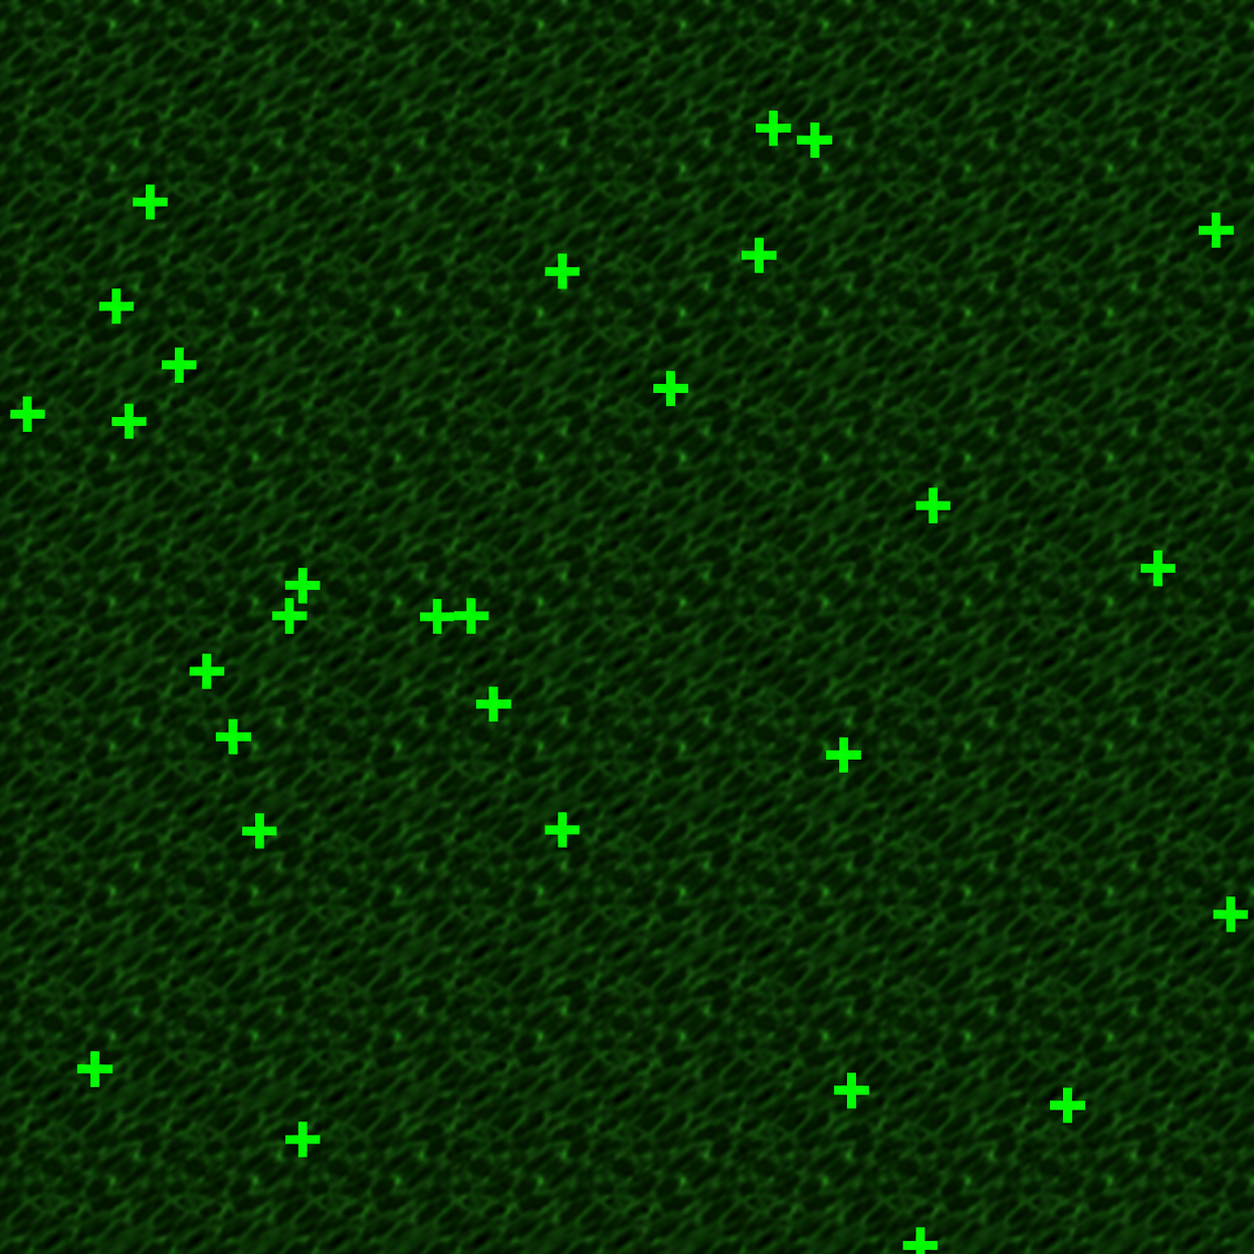
\includegraphics[width=0.5\linewidth]{figuras/top-down-health-gathering.png}
    \caption{Visão superior do ambiente da tarefa \textit{Health-Gathering}. Os itens em formato de ``+'' representam os \textit{medikits} distribuídos no ambiente, que podem ser coletados pelo agente para restaurar sua vida.\\
    \textbf{Fonte:} Elaborada pelo autor}
    \label{fig:health-gathering-topdown}
\end{figure}


Além disso, o \textit{Health-Gathering} permite formular uma tarefa visual de navegação e forrageamento. O agente percebe o ambiente por meio de imagens da tela e deve selecionar ações que o mantenham em interação com o mundo. Essa característica aproxima o problema de tarefas de Aprendizado por Reforço Profundo baseadas em percepção visual, ao mesmo tempo em que fornece uma estrutura simples para investigar sobrevivência, busca por recursos e adaptação.

No contexto do VizDoom, um \textit{tick} corresponde a uma unidade discreta de atualização do jogo. A cada \textit{tick}, o ambiente atualiza seus elementos internos, como posição do agente, estado dos objetos, valor de vida e observação visual disponível. Assim, o episódio pode ser entendido como uma sequência finita de \textit{ticks}, durante os quais o agente observa o ambiente, escolhe ações e sofre as consequências dessas ações. Na configuração experimental adotada, cada episódio terá duração máxima de 2100 \textit{ticks}.

A vida do agente funciona apenas como uma variável de controle do ambiente. Seu valor não compõe a observação fornecida à política, não é utilizado no cálculo da recompensa e não participa diretamente da atualização do aprendizado. Quando a vida chega a zero, o ambiente encerra o episódio, simulando a morte do agente após permanecer tempo suficiente sem se alimentar. Dessa forma, a vida determina por quanto tempo a interação pode continuar, mas não informa ao agente qual comportamento deve ser aprendido.

A perda de vida ocorre continuamente porque o chão do ambiente é ácido. O agente inicia cada episódio com 100 pontos de vida, que também correspondem à sua vida máxima, e perde 8 pontos de vida a cada 36 \textit{ticks}, independentemente da ação escolhida. Os \textit{medikits} funcionam como recursos de recuperação: ao serem coletados, restauram 25 pontos de vida do agente. O ambiente conterá 16 \textit{medikits} disponíveis simultaneamente, posicionados aleatoriamente no início do episódio. Novos \textit{medikits} surgirão a cada 30 \textit{ticks} do jogo, mantendo a dinâmica de busca por recursos ao longo do episódio.

Os principais elementos do ambiente padrão, portanto, incluem a vida inicial e máxima do agente, a duração máxima dos episódios, a taxa de perda de vida no chão ácido, a quantidade de \textit{medikits} disponíveis, a quantidade de vida restaurada por cada item e a regra de surgimento dos novos \textit{medikits}. Esses elementos definem a dinâmica básica de sobrevivência e coleta de recursos da tarefa \textit{Health-Gathering}.

\section{Formulação em Aprendizado por Reforço}

Como discutido na Seção~\ref{subsec:aprendizado-por-reforco}, o Aprendizado por Reforço modela a interação entre agente e ambiente como um processo sequencial de observação, ação, transição de estado e recompensa. Nesta pesquisa, a tarefa \textit{Health-Gathering} será formulada a partir dessa estrutura: a cada instante de tempo, o agente recebe uma observação visual do ambiente, escolhe uma ação e recebe um sinal de recompensa. Em seguida, o ambiente é atualizado e uma nova observação é produzida. Esse ciclo se repete até o fim do episódio, que pode ocorrer quando a vida do agente chega a zero ou quando o limite máximo de \textit{ticks} é atingido.

\subsection{Observação}

As observações serão compostas por imagens do ponto de vista do agente. Assim, o agente não receberá uma representação simbólica do ambiente, como coordenadas absolutas dos \textit{medikits} ou mapas completos da sala, mas sim informações visuais para um personagem situado no ambiente.

As imagens passarão por uma sequência fixa de pré-processamento, ilustrada na Figura~\ref{fig:preprocessamento-observacao}. A observação original fornecida pelo ambiente possui resolução de $320 \times 240$ pixels em RGB. Em seguida, a imagem será convertida para escala de cinza, reduzindo os três canais de cor a um único canal de intensidade. Depois, será redimensionada para $84 \times 84$ pixels. Por fim, os valores dos pixels serão divididos por $255$, passando inicialmente para o intervalo $[0,1]$. Durante o treinamento, o Sample Factory também aplica uma normalização estatística baseada na média e no desvio padrão acumulados das observações.

O treinamento diretamente com as imagens originais exigiria processar uma quantidade muito maior de valores a cada interação, aumentando o consumo de memória, o tempo de inferência e o custo das atualizações da rede. Além disso, as informações de cor e a alta resolução não são indispensáveis para distinguir os principais elementos desta tarefa, como paredes, regiões navegáveis e \textit{medikits}. O pré-processamento reduz detalhes visuais que não são centrais para o experimento, padroniza a escala da entrada e permite coletar e processar mais experiências com os recursos computacionais disponíveis. A resolução de $84 \times 84$ preserva a estrutura espacial necessária à navegação e à identificação dos recursos, sem impor o custo de treinar com a imagem original. Essa escolha, portanto, busca eficiência e estabilidade no treinamento, e não a obtenção da representação visual mais detalhada possível.

\begin{figure}[h!]
    \centering
    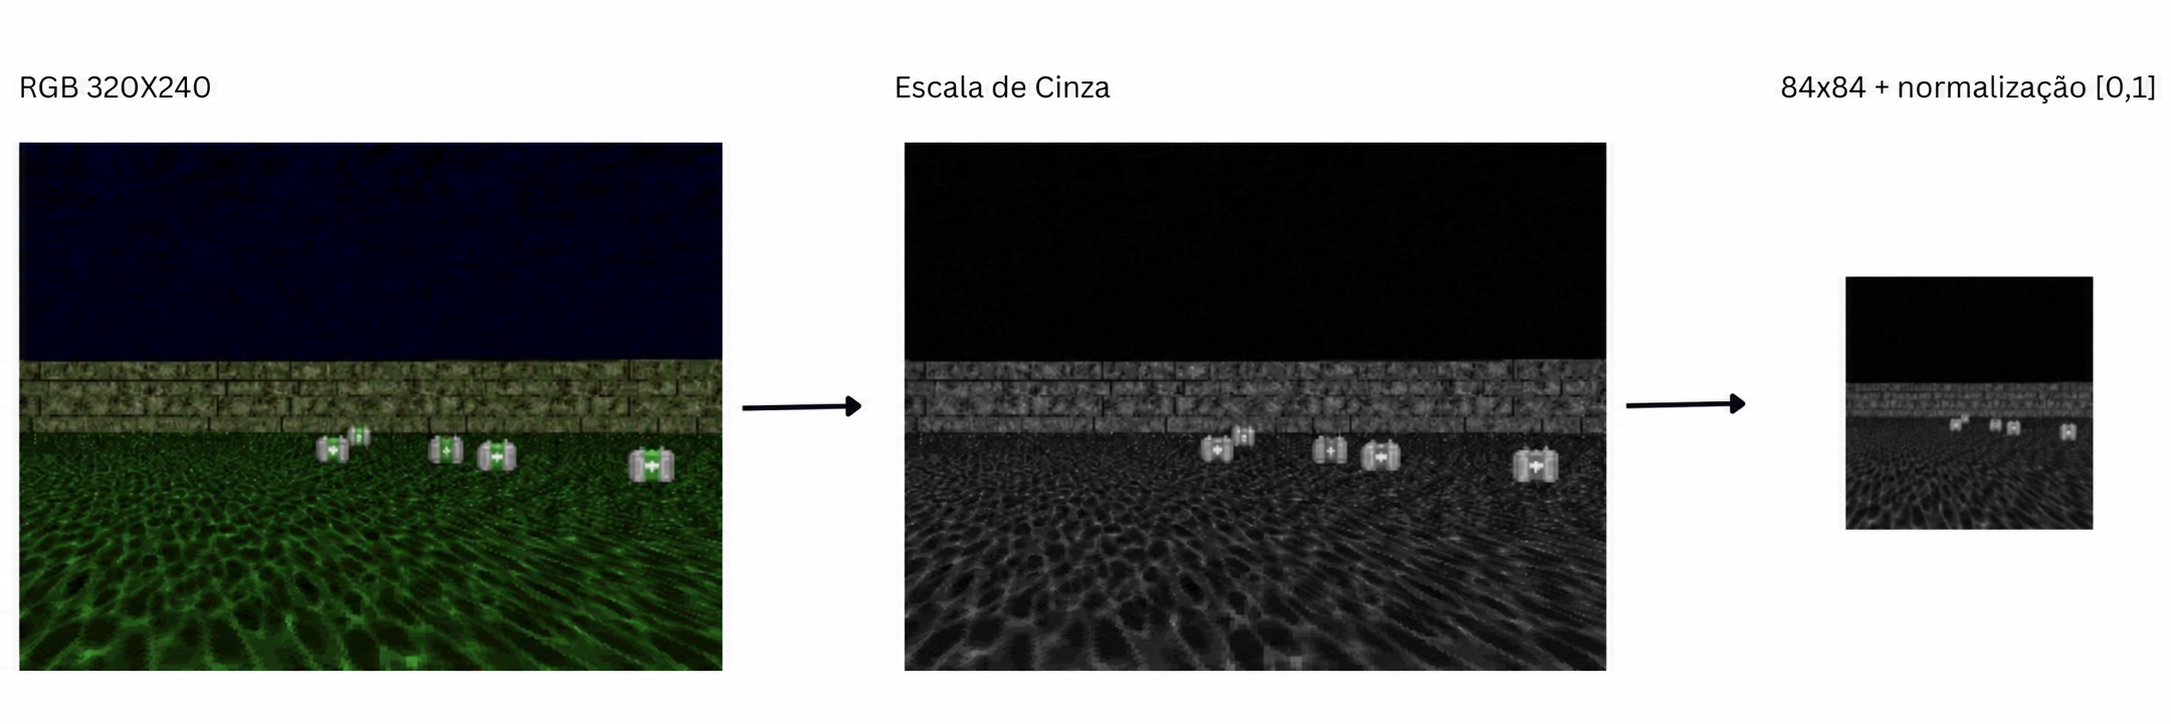
\includegraphics[width=1.0\linewidth]{figuras/preprocessamento-observacao.png}
    \caption{Etapas de pré-processamento da observação visual do agente: imagem RGB original com resolução de $320 \times 240$ pixels, conversão para escala de cinza, redimensionamento para $84 \times 84$ pixels e normalização dos valores para o intervalo $[0,1]$.\\
    \textbf{Fonte:} Elaborada pelo autor}
    \label{fig:preprocessamento-observacao}
\end{figure}

\subsection{Ação}

O conjunto de ações será composto por três comandos discretos de navegação: ir em frente, virar à esquerda e virar à direita. Essas ações permitem que o agente explore a sala e se desloque em direção aos recursos disponíveis, mantendo a formulação do problema simples e adequada aos objetivos da pesquisa.

A ação de andar para trás foi omitida por ser redundante, pois o agente pode girar e avançar na direção oposta. Essa simplificação reduz o espaço de ações e afeta igualmente todas as condições experimentais.


\subsection{Recompensa}

Na tarefa \textit{Health-Gathering}, o agente recebe uma recompensa extrínseca de $+0{,}01$ a cada \textit{tick} e de $+1$ para cada \textit{medikit} utilizado. Essa formulação incentiva tanto a permanência no ambiente quanto o uso dos recursos responsáveis pela recuperação da vida.

Neste trabalho, entretanto, essa recompensa extrínseca será zerada. Essa decisão evita que a solução do problema seja introduzida diretamente na função de recompensa e permite investigar formas alternativas de orientação comportamental. A recompensa utilizada nos experimentos será detalhada nos próximos capítulos, especialmente na discussão sobre motivação intrínseca e curiosidade artificial.


\section{Algoritmo de Aprendizado}

A política do agente será treinada a partir do mecanismo de atualização do \textit{Proximal Policy Optimization} (PPO). Como apresentado na Seção~\ref{subsubsec:ppo}, o PPO busca atualizar a política de forma estável, evitando mudanças abruptas entre a política usada para coletar experiências e a nova política aprendida.

A implementação do treinamento utiliza a biblioteca Sample Factory \cite{sample_factory}, que fornece uma arquitetura assíncrona e de alto desempenho para algoritmos de Aprendizado por Reforço. Enquanto o PPO fornece o mecanismo de atualização da política, o Sample Factory paraleliza a coleta de experiências em múltiplas instâncias do ambiente e separa os componentes responsáveis pela simulação, pela inferência da política e pela atualização da rede. O treinamento deixa, assim, de depender de uma execução estritamente sequencial entre coleta de dados e otimização.

Essa arquitetura foi escolhida por sua elevada eficiência no aproveitamento dos recursos computacionais. A execução assíncrona reduz períodos de ociosidade, permite utilizar simultaneamente múltiplos núcleos de CPU para simular ambientes e agrupa inferências e atualizações na GPU. O Sample Factory foi projetado para alcançar alto volume de interações em uma única máquina e em hardware amplamente disponível, evitando a necessidade de grandes infraestruturas distribuídas \cite{sample_factory}. Embora o desempenho efetivo dependa da configuração utilizada, essa eficiência torna viável realizar milhões de passos de interação e repetir treinamentos em equipamentos menos robustos. Neste trabalho, o PPO define o mecanismo de otimização da política, enquanto o Sample Factory fornece a infraestrutura utilizada para executar o treinamento de forma paralela e eficiente.

Nesta seção, serão descritos os principais elementos necessários para a implementação do algoritmo de aprendizado, incluindo os hiperparâmetros utilizados e a arquitetura da rede neural.

\subsection{Hiperparâmetros}

O Sample Factory oferece numerosos parâmetros de configuração, mas nem todos são relevantes para a descrição metodológica. A Tabela~\ref{tab:hiperparametros-ppo} reúne os parâmetros que afetam diretamente a atualização da política, a estimativa dos retornos e a estabilidade do aprendizado.

\begin{table}[h!]
\centering
\small
\caption{Hiperparâmetros de aprendizado utilizados no PPO.}
\label{tab:hiperparametros-ppo}
\begin{tabular}{l|l|p{7cm}}
\hline
\textbf{Parâmetro} & \textbf{Valor} & \textbf{Descrição} \\
\hline
\texttt{batch\_size} & $1024$ & Número de transições em cada minilote de otimização. \\
\texttt{num\_epochs} & $1$ & Número de passagens de otimização sobre cada conjunto de experiências coletado. \\
\texttt{learning\_rate} & $0{,}0001$ & Magnitude das atualizações realizadas pelo otimizador. \\
\texttt{gamma} & $0{,}999$ & Fator de desconto aplicado às recompensas futuras. \\
\texttt{ppo\_clip\_ratio} & $0{,}1$ & Limita a alteração da política entre atualizações consecutivas. \\
\texttt{ppo\_clip\_value} & $0{,}2$ & Limita a alteração da estimativa produzida pela função de valor. \\
\hline
\end{tabular}
\end{table}

\subsection{Arquitetura da Rede Neural}

A arquitetura da rede neural será responsável por transformar a observação visual pré-processada em uma representação latente utilizada pela política do agente. Como a entrada é uma imagem em escala de cinza, o modelo utiliza um codificador convolucional. A Tabela~\ref{tab:arquitetura-rede-ppo} apresenta a arquitetura utilizada.

\begin{table}[h!]
\centering
\caption{Arquitetura da rede neural utilizada pelo agente.}
\label{tab:arquitetura-rede-ppo}
\begin{tabular}{c|l|l|l}
\hline
\textbf{Etapa} & \textbf{Camada} & \textbf{Configuração} & \textbf{Saída} \\
\hline
1 & Convolucional 2D & $1 \rightarrow 32$, kernel $8 \times 8$, stride $4 \times 4$ & 32 mapas de características \\
2 & ReLU &  & 32 mapas de características \\
3 & Convolucional 2D & $32 \rightarrow 64$, kernel $4 \times 4$, stride $2 \times 2$ & 64 mapas de características \\
4 & ReLU &  & 64 mapas de características \\
5 & Convolucional 2D & $64 \rightarrow 128$, kernel $3 \times 3$, stride $2 \times 2$ & 128 mapas de características \\
6 & ReLU &  & 128 mapas de características \\
7 & Flatten & Vetorização das ativações & 2048 unidades \\
8 & Linear & $2048 \rightarrow 512$ & 512 unidades \\
9 & ReLU &  & 512 unidades \\
10 & Política (linear) & $512 \rightarrow 4$ & 4 valores de ação \\
\hline
\end{tabular}
\end{table}

A Figura~\ref{fig:arquitetura-politica} apresenta uma representação visual do fluxo de processamento da política, desde a observação de entrada até os valores associados às ações.

\begin{figure}[h!]
    \centering
    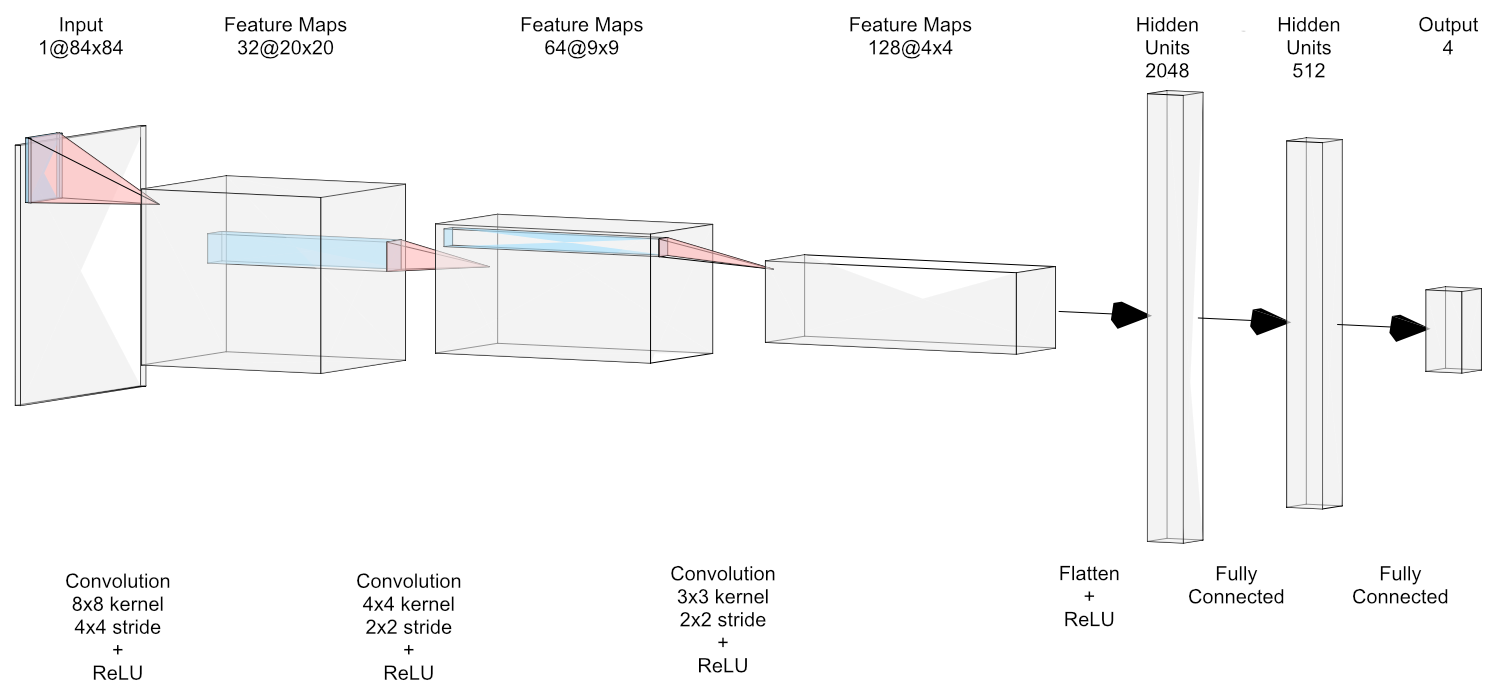
\includegraphics[width=1.0\linewidth]{figuras/policy_architecture.png}
    \caption{Arquitetura da rede neural utilizada pela política do agente, composta por três camadas convolucionais, uma etapa de vetorização, uma camada totalmente conectada com 512 unidades e a camada de saída.\\
    \textbf{Fonte:} Elaborada pelo autor.}
    \label{fig:arquitetura-politica}
\end{figure}

O codificador convolucional extrai características espaciais da observação visual, enquanto a camada linear projeta essas características para uma representação compacta de 512 unidades. A primeira camada não convolucional utiliza essa representação para produzir os valores associados às ações disponíveis para a política.

A escolha dessa arquitetura convolucional é deliberadamente simples. O objetivo dos experimentos não é obter o melhor desempenho possível na tarefa nem propor uma nova arquitetura de percepção, mas avaliar, de maneira controlada, o efeito geral da relação entre glaucoma artificial, curiosidade e viabilidade. Para esse propósito, a CNN é suficiente para extrair características espaciais relevantes das observações e fornecer à política informações necessárias à navegação e à identificação de recursos. Técnicas mais sofisticadas não foram consideradas porque acrescentariam componentes desnecessários para o objetivo do trabalho. Assim, a arquitetura adotada privilegia simplicidade, sem pretensão de alcançar o estado da arte em desempenho.

\section{Configuração Experimental do Treinamento}

Todos os experimentos utilizarão a mesma configuração básica de observação e execução, apresentada na Tabela~\ref{tab:configuracao-execucao}. Cada treinamento será realizado por $10\,000\,000$ de passos de interação com o ambiente. A adoção do mesmo limite em todas as condições garante que os agentes disponham do mesmo orçamento de experiência, permitindo atribuir as diferenças observadas às formas de recompensa e aos níveis de glaucoma, em vez de a durações distintas de treinamento.

Para acelerar a geração dessas experiências, foram utilizados $4$ processos paralelos, definidos pelo parâmetro \texttt{num\_workers}. Cada processo executa duas instâncias independentes do ambiente, conforme definido por \texttt{num\_envs\_per\_worker}, totalizando até $8$ instâncias em execução simultânea. Essa configuração permite coletar transições de diferentes episódios ao mesmo tempo, aproveitando melhor os núcleos da CPU e reduzindo o tempo necessário para alcançar os $10\,000\,000$ de passos. Esses parâmetros alteram a velocidade de coleta das experiências, mas não o número total de passos nem o objetivo de aprendizado do agente.

Também foi utilizado \texttt{env\_frameskip} igual a $4$. Com essa configuração, cada ação escolhida pelo agente é mantida durante quatro quadros consecutivos do ambiente antes que uma nova decisão seja calculada. Isso reduz a frequência de inferências da rede neural e a quantidade de observações que precisam ser processadas para avançar o mesmo intervalo de tempo no jogo, acelerando a simulação e o treinamento. Embora valores maiores possam eliminar mudanças visuais importantes entre duas decisões, o valor $4$ oferece um equilíbrio entre eficiência computacional e controle do agente. Como o mesmo valor é empregado em todas as condições experimentais, seus efeitos permanecem constantes nas comparações realizadas.

\begin{table}[h!]
\centering
\small
\caption{Configurações de execução do treinamento.}
\label{tab:configuracao-execucao}
\begin{tabular}{l|l|p{7cm}}
\hline
\textbf{Parâmetro} & \textbf{Valor} & \textbf{Descrição} \\
\hline
\texttt{env\_frameskip} & $4$ & Mantém cada ação durante quatro quadros consecutivos do ambiente. \\
\texttt{num\_workers} & $4$ & Número de processos utilizados para executar ambientes em paralelo. \\
\texttt{num\_envs\_per\_worker} & $2$ & Número de instâncias do ambiente executadas por cada processo. \\
\texttt{train\_for\_env\_steps} & $10\,000\,000$ & Número total de passos de interação realizados em cada experimento. \\
\hline
\end{tabular}
\end{table}

\section{Estratégia de Recompensa}
\label{sec:estrategia-recompensa}

\subsection{O Problema da Recompensa}
\label{subsec:problema-recompensa}

A escolha da recompensa é um dos pontos centrais desta proposta metodológica. Um personagem artificial considerado inteligente não deve apenas repetir um comportamento fixo independentemente do que ocorre ao seu redor. Pelo contrário, espera-se que ele seja capaz de perceber mudanças no ambiente, compreender a dinâmica da situação em que está inserido e agir de maneira flexível. Nesse sentido, a inteligência não é entendida apenas como a execução eficiente de uma ação previamente desejada, mas como a capacidade de encontrar formas de ação adequadas diante de diferentes condições.

Reforçar diretamente um comportamento específico tende a produzir agentes que executam apenas aquele comportamento. Embora isso possa resolver uma tarefa delimitada, também pode tornar o agente monótono e limitar a descoberta de soluções melhores, que talvez não tenham sido previstas pelo projetista durante a engenharia de recompensas. Assim, quando a recompensa força uma solução, ela pode impedir que o agente explore outras possibilidades de ação que também resolveriam o problema, ou até o resolveriam de maneira mais robusta.

Esse problema retoma a discussão apresentada na fundamentação teórica sobre Aprendizado por Reforço, na qual a recompensa aparece como o sinal que orienta a atualização da política do agente (Seção~\ref{subsec:aprendizado-por-reforco}). Como o agente aprende a maximizar a recompensa acumulada, a forma como esse sinal é definido não é um detalhe apenas técnico, pois ela delimita o que será considerado desejável dentro do processo de aprendizagem. Por isso, a engenharia de recompensas pode resolver tarefas específicas, mas também pode introduzir diretamente a solução esperada pelo projetista.

Essa distinção conduz ao problema conceitual discutido na fundamentação filosófica. Se a inteligência pode ser entendida como um fenômeno emergente da vida, isto é, como algo que surge de uma organização capaz de manter a si mesma em relação contínua com o ambiente (Seção~\ref{subsec:inteligencia-fenomeno-emergente-vida}), então não basta associar a palavra ``vida'' a uma variável numérica do ambiente. Em Aprendizado por Reforço, o agente não está propriamente trabalhando para se manter vivo. O que ele faz é maximizar um sinal numérico de recompensa acumulada. Mesmo quando a recompensa está associada ao tempo de sobrevivência, o agente não compreende esse número como vida. Para o algoritmo, trata-se apenas de um valor a ser aumentado.

Assim, dizer que o agente ``quer sobreviver'' é apenas uma metáfora. O problema em si não possui significado para ele, a menos que a própria organização do agente e de sua interação com o ambiente produza algum domínio de relevância. Por isso, recompensar diretamente a coleta de \textit{medikits}, a navegação até uma região ou o tempo de sobrevivência resolveria parte do problema experimental, mas manteria a orientação do comportamento inteiramente dependente de uma especificação externa. A proposta, portanto, não é eliminar a recompensa, pois ela continua sendo necessária ao funcionamento do Aprendizado por Reforço, mas deslocar seu papel, para que, em vez de funcionar como uma instrução direta sobre qual ação executar, ela favoreça a exploração e a busca por soluções.

\subsection{Autopoiese, IA Enativa e Perspectiva de Solução}
\label{subsec:autopoiese-ia-enativa-solucao}

É nesse ponto que a Inteligência Artificial Enativa oferece uma motivação conceitual importante. Na perspectiva de \citeonline{maturana1980autopoiesis}, a vida não é apenas a posse de uma variável chamada vida, mas uma dinâmica de autoprodução e manutenção de uma unidade que se diferencia do ambiente. Um ser vivo existe porque há uma dinâmica interna que trabalha continuamente para manter sua própria organização. Essa dinâmica depende do ambiente, pois os recursos necessários à sua continuidade precisam ser encontrados e incorporados. Por isso, a vida possui uma dimensão intencional, na qual o organismo se orienta no ambiente a partir daquilo que importa para a manutenção de sua própria existência.

A noção de autopoiese permite compreender essa relação. Um sistema autopoiético é uma dinâmica que produz e mantém a si mesma, distinguindo-se do meio em que está inserida. Essa manutenção, porém, não está garantida de antemão. O sistema permanece exposto a perturbações e depende de condições de viabilidade para continuar existindo. Neste trabalho, precariedade designa essa dependência contínua de condições que podem ser perdidas. Um sistema é precário quando sua organização não está assegurada e precisa ser constantemente mantida por meio de sua própria atividade e de suas interações com o ambiente. Portanto, precariedade não significa apenas fragilidade ou dificuldade imposta externamente. Ela corresponde à possibilidade de que determinadas perturbações comprometam a continuidade da organização do próprio sistema.

Essa definição pode ser aproximada da noção de idiossincrasia, entendida como uma predisposição particular do organismo que faz com que ele responda de maneira própria à influência de agentes externos. Um mesmo elemento do ambiente pode produzir efeitos diferentes conforme a organização e a condição interna daquele que o encontra. Dessa maneira, o valor de uma interação não pertence exclusivamente ao objeto externo, mas emerge da relação entre esse objeto e as necessidades particulares do sistema. A precariedade fornece, assim, a condição pela qual certas perturbações adquirem relevância, enquanto a idiossincrasia ajuda a compreender por que essa relevância depende da constituição específica do agente.

Em termos de viabilidade, a precariedade pode ser compreendida pela proximidade de um sistema em relação à fronteira além da qual sua organização não pode mais ser mantida. Quanto mais próximo dessa fronteira um indivíduo se encontra, mais precária é sua condição, pois menor é sua margem para absorver perturbações sem comprometer sua continuidade. Inversamente, quanto mais distante da fronteira de viabilidade, maior é sua margem de estabilidade. A precariedade não constitui, portanto, uma propriedade simplesmente presente ou ausente, mas uma condição gradual e dinâmica que varia conforme o estado do indivíduo e sua relação com o ambiente.

Com base nessa leitura, a perspectiva de solução adotada neste trabalho consiste em introduzir uma forma artificial de precariedade no agente. A função dessa precariedade é fazer com que a condição interna do agente tenha consequências sobre sua relação com o ambiente. Em vez de dizer diretamente que coletar \textit{medikits} é desejável, busca-se criar uma dinâmica em que ficar muito tempo sem recuperar sua condição interna afete suas possibilidades de perceber, explorar e continuar interagindo.

Dessa forma, a precariedade serve como mediação entre a condição interna do agente, sua relação com o ambiente e suas ações. Ela transforma a viabilidade em uma condição prática para a continuidade da interação. A coleta de recursos pode então tornar-se relevante não porque foi imposta como objetivo final pela função de recompensa, mas porque contribui para afastar o agente da fronteira de viabilidade e preservar suas possibilidades de ação.

A questão metodológica passa a ser, portanto, como introduzir a precariedade no agente. Se a proposta é fazer com que a condição interna afete a própria relação perceptiva com o ambiente, é necessário definir um mecanismo capaz de degradar e recuperar a percepção de acordo com essa condição. No experimento proposto, esse papel será desempenhado pelo glaucoma artificial, apresentado na seção seguinte.


\section{Glaucoma como Precariedade}
\label{sec:glaucoma-precariedade}

O glaucoma é um conjunto de doenças oculares que danificam o nervo óptico, estrutura responsável por transmitir ao cérebro as informações captadas pelo olho. Em suas formas mais comuns, a perda visual tende a ocorrer lentamente e pode não ser percebida em seus estágios iniciais. O comprometimento geralmente começa pela visão periférica e pode avançar para o estreitamento do campo visual, produzindo uma percepção semelhante à visão em túnel. Em estágios avançados, a doença pode atingir a visão central e causar perda visual irreversível ou cegueira \cite{nei-glaucoma}. A Figura~\ref{fig:glaucoma-visao-humana} apresenta uma comparação ilustrativa entre uma visão sem comprometimento e a perda de visão periférica associada ao glaucoma.

\begin{figure}[h!]
    \centering
    
\includegraphics[width=0.9\linewidth]{figuras/glaucoma_human.jpg}
    \caption{Comparação ilustrativa entre uma visão sem comprometimento, à esquerda, e a perda de visão periférica associada ao glaucoma, à direita.\\
    \textbf{Fonte:} American Optometric Association \cite{aoa-glaucoma}.}
    \label{fig:glaucoma-visao-humana}
\end{figure}

\subsection{Glaucoma Artificial}

A forma de precariedade artificial proposta neste trabalho foi inspirada no comprometimento do campo visual causado pelo glaucoma apresentado anteriormente. Essa inspiração, entretanto, não corresponde a uma reprodução clínica da doença. Enquanto o glaucoma humano costuma comprometer inicialmente a visão periférica, o glaucoma artificial adotado no experimento começa no centro da observação e se expande progressivamente em direção às bordas. O termo é utilizado, portanto, como uma analogia para representar uma perda gradual da capacidade visual, e não como uma simulação fisiologicamente fiel do glaucoma.

O glaucoma artificial é o mecanismo escolhido para materializar uma forma específica da precariedade discutida na seção anterior. Neste experimento, ele é compreendido como precariedade perceptiva, pois a aproximação da fronteira de viabilidade se manifesta pela perda progressiva das condições de percepção do agente. Enquanto o agente permanece sem coletar \textit{medikits}, sua visão se degrada gradualmente. Quando coleta um \textit{medikit}, essa degradação é removida. Desse modo, a precariedade não aparece apenas como uma penalidade externa na função de recompensa, mas atua diretamente sobre a forma como o agente acessa o ambiente.

Essa escolha é importante porque conecta o problema da recompensa à perspectiva enativa adotada neste trabalho. Se o agente recebesse uma recompensa direta por coletar \textit{medikits}, o comportamento esperado estaria explicitamente especificado pelo projetista. Com o glaucoma artificial, por outro lado, a coleta de recursos passa a ter importância indireta, pois preserva as condições perceptivas necessárias para que o agente continue explorando o ambiente. Assim, o glaucoma funciona como uma forma computacional de precariedade, pois traduz a passagem do tempo sem recuperação interna em perda progressiva de capacidade perceptiva.

A Figura~\ref{fig:glaucoma-visao-agente} ilustra a evolução do efeito visual esperado em quatro momentos. A primeira imagem apresenta a visão limpa do agente, após $0$ \textit{frames} sem comer, ou seja, o agente acabou de usar um \textit{medikit}. A segunda mostra um glaucoma inicial, após $1$ \textit{frame} sem comer. A terceira mostra uma degradação mais acentuada, após $20$ \textit{frames} sem comer. A quarta e última mostra uma degradação severa, após $50$ \textit{frames} sem comer. Esse tipo de transformação representa a ideia de que um agente em pior condição interna não deixa apenas de receber pontos, mas passa a perceber o mundo de modo mais limitado.

\begin{figure}[h!]
    \centering
    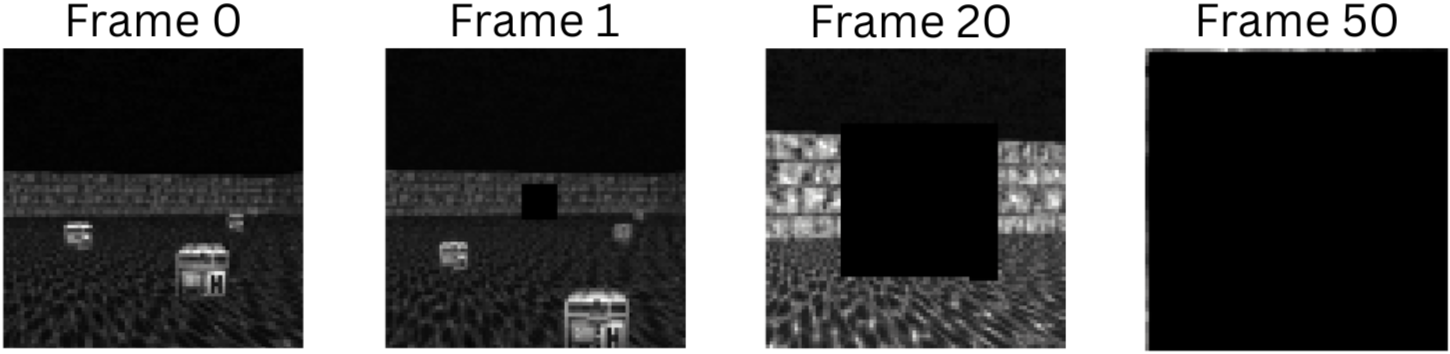
\includegraphics[width=0.9\linewidth]{figuras/glaucoma-evolution.png}
    \caption{Evolução da percepção visual do agente com glaucoma artificial de força 100. Da esquerda para a direita, a figura mostra a visão limpa após $0$ \textit{frames} sem comer, glaucoma inicial após $1$ \textit{frame}, degradação intermediária após $20$ \textit{frames} e degradação severa após $50$ \textit{frames}.\\
    \textbf{Fonte:} Elaborada pelo autor}
    \label{fig:glaucoma-visao-agente}
\end{figure}

Do ponto de vista implementacional, a velocidade de crescimento do glaucoma será controlada por uma variável do programa, chamada força do glaucoma. Essa variável define quantos pixels passam a sofrer degradação a cada \textit{tick} em que o agente permanece sem coletar um \textit{medikit}. Por exemplo, se a força do glaucoma tiver valor $100$, então, a cada \textit{tick} sem comer, mais $100$ pixels serão afetados pelo glaucoma. De modo geral, se a força do glaucoma tiver valor $x$, então o glaucoma crescerá $x$ pixels por \textit{tick} sem recuperação. Quando o agente coleta um \textit{medikit}, o nível de glaucoma é reiniciado e a percepção volta ao estado sem degradação.

Os pixels afetados pelo glaucoma seguem um padrão espacial definido do centro para as bordas da imagem. A degradação começa ao redor do ponto central da observação e se expande progressivamente formando um quadrado em torno de si mesmo. A cada atualização, novos pixels são incorporados à região degradada, aumentando o tamanho desse quadrado pixel a pixel. Dessa forma, o glaucoma não surge aleatoriamente na imagem, mas cresce de maneira ordenada, produzindo uma perda visual progressiva e espacialmente estruturada.

Formalmente, a evolução do glaucoma pode ser representada por uma variável $g_t$, que indica a quantidade acumulada de pixels afetados no instante $t$. Se o agente não coleta um \textit{medikit}, então $g_{t+1}=g_t+x$, em que $x$ representa a força do glaucoma definida no programa. Se ocorre a coleta, então $g_{t+1}=0$. Esse valor determina o tamanho da região quadrada degradada aplicada à observação antes que ela seja entregue à rede neural do agente.

Com isso, o glaucoma estabelece uma relação direta entre estado interno e percepção. Quanto maior o tempo sem recuperação, maior a degradação visual. Quanto mais cedo o agente encontra um recurso, mais rapidamente recupera sua percepção. A hipótese metodológica é que essa relação possa favorecer comportamentos adaptativos sem que a coleta de \textit{medikits} precise ser recompensada diretamente. O modo proposto para transformar essa precariedade corporal em sinal de recompensa será apresentado na seção seguinte, por meio de recompensa intrínseca baseada em curiosidade e implementada com RND.

\section{Recompensa Intrínseca por Curiosidade}
\label{sec:recompensa-intrinseca-curiosidade}

Esta seção apresenta o ponto em que a precariedade corporal introduzida pelo glaucoma artificial é transformada em sinal de recompensa. Como discutido na Seção~\ref{subsec:problema-recompensa}, o agente de Aprendizado por Reforço não age porque compreende a vida ou a sobrevivência como valores próprios. Ele ajusta sua política para maximizar uma recompensa acumulada, conforme a formulação de Aprendizado por Reforço apresentada na Seção~\ref{subsec:aprendizado-por-reforco}. Por isso, a contribuição metodológica deste trabalho consiste em deslocar a recompensa de uma instrução direta, como coletar \textit{medikits}, para uma consequência indireta da precariedade corporal.

A ideia central é que quanto mais precário estiver o corpo artificial do agente, menor deve ser a recompensa obtida por sua interação com o ambiente. De modo complementar, quanto menos precário estiver esse corpo, maior tende a ser a recompensa. Com isso, o agente não é recompensado diretamente por estar vivo ou por coletar um recurso específico. Ele é levado a buscar condições menos precárias porque essas condições preservam sua capacidade de perceber um ambiente mais rico e informativo. Assim, a recompensa passa a favorecer a manutenção do agente dentro de restrições de viabilidade, retomando a discussão sobre autopoiese, precariedade e IA Enativa desenvolvida na Seção~\ref{subsec:autopoiese-ia-enativa-solucao}.

Essa formulação também dialoga com os trabalhos relacionados discutidos no Capítulo~\ref{cap:trabalhos-relacionados}. Em particular, trabalhos de Aprendizado por Reforço Profundo mostraram a eficácia de agentes treinados a partir de entradas visuais e recompensas escalares, mas permaneceram fortemente dependentes de objetivos externos definidos pelo ambiente ou pelo projetista. Já trabalhos relacionados à autonomia e à motivação intrínseca indicam a importância de sinais internos para orientar o comportamento, mas ainda deixam em aberto como relacionar esses sinais a uma condição corporal de precariedade. Este trabalho procura ocupar justamente esse espaço, articulando percepção degradada, viabilidade e recompensa.

A recompensa total utilizada pelo agente será definida como a soma entre recompensa extrínseca e recompensa intrínseca, conforme a formulação discutida na fundamentação teórica sobre recompensa intrínseca:

$$
r_t = r_t^{\text{ext}} + r_t^{\text{int}}.
$$

Neste experimento, entretanto, a recompensa extrínseca será zerada, como definido na Subseção~\ref{subsec:problema-recompensa} e na formulação da recompensa do ambiente. Assim, tem-se:

$$
r_t^{\text{ext}} = 0
$$

\noindent e, consequentemente:

$$
r_t = r_t^{\text{int}}.
$$

\subsection{Calculando a Recompensa Intrínseca}

A recompensa intrínseca será calculada por meio do método \textit{Random Network Distillation} (RND), apresentado na Seção~\ref{subsubsec:rnd}. No RND, uma rede alvo fixa produz uma representação da observação, enquanto uma rede preditora tenta aproximar essa representação. O erro de predição entre essas redes funciona como medida de novidade. Observações mais ricas, variadas ou menos conhecidas tendem a produzir maior erro de predição e, portanto, maior recompensa intrínseca.

As redes alvo e preditora possuem a mesma arquitetura, apresentada na Figura~\ref{fig:arquitetura-rnd} e detalhada na Tabela~\ref{tab:arquitetura-rnd}. Ambas recebem como entrada a observação pré-processada em escala de cinza, com resolução de $84 \times 84$ pixels, e produzem um vetor de características com 512 unidades. A diferença entre elas não está na estrutura, mas no processo de aprendizado: os parâmetros da rede alvo são inicializados aleatoriamente e permanecem fixos, enquanto os parâmetros da rede preditora são atualizados para aproximar a representação produzida pela rede alvo.

\begin{figure}[h!]
    \centering
    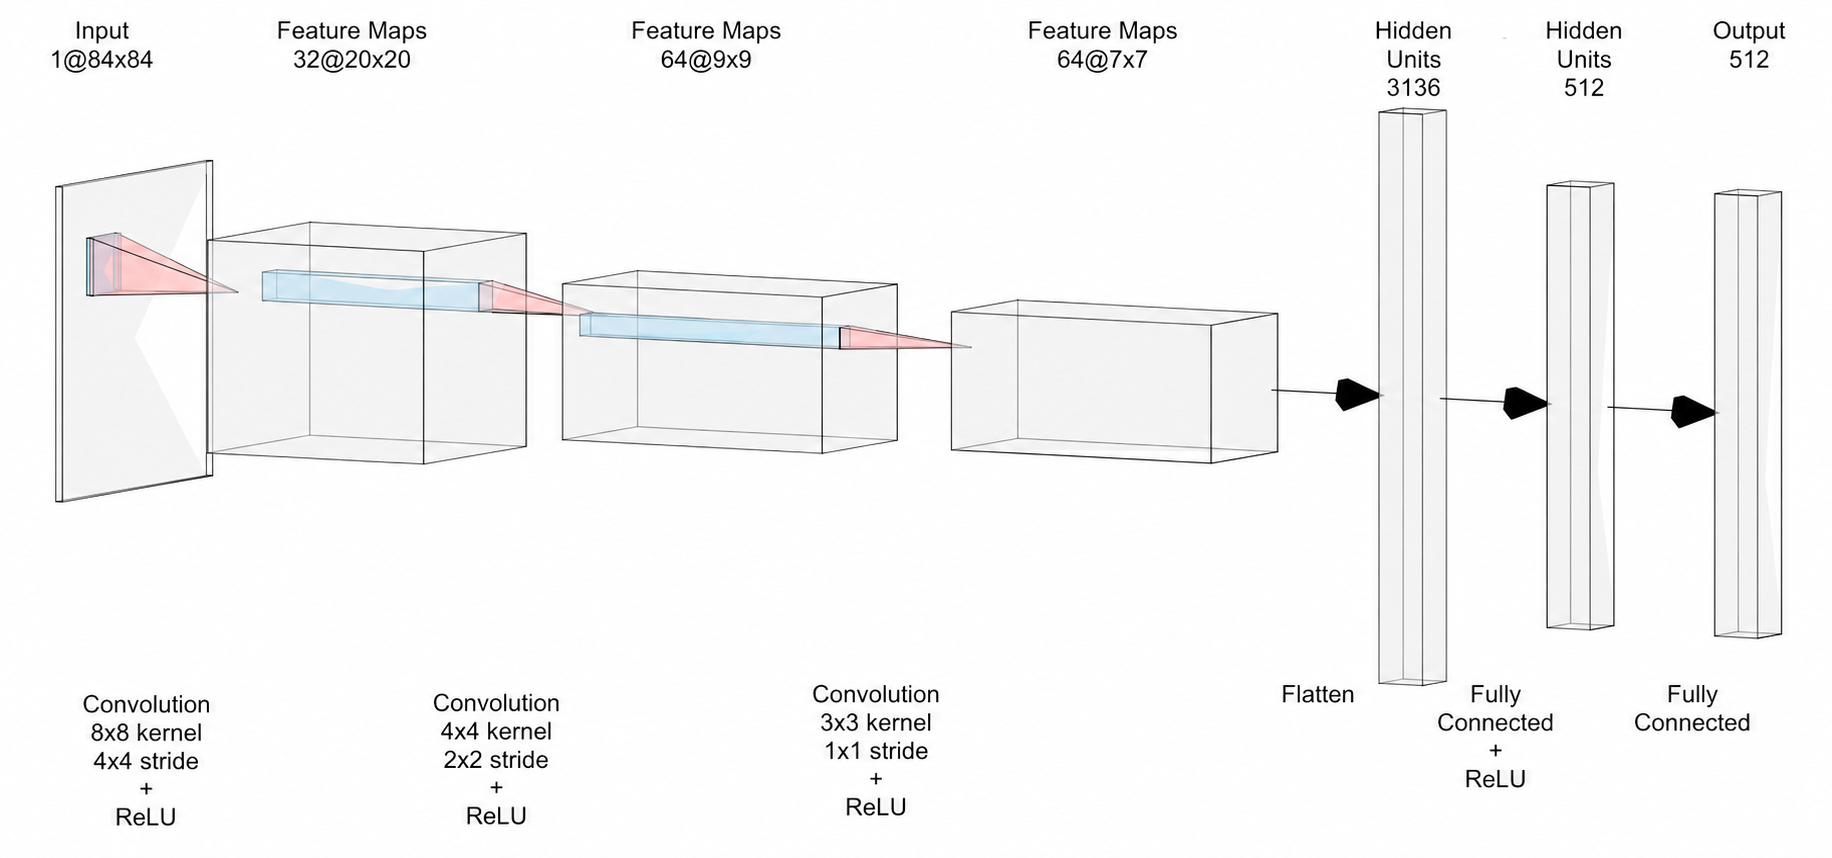
\includegraphics[width=1.0\linewidth]{figuras/rnd_architecture.png}
    \caption{Arquitetura compartilhada pelas redes alvo e preditora do RND, composta por três camadas convolucionais, uma etapa de vetorização e duas camadas totalmente conectadas.\\
    \textbf{Fonte:} Elaborada pelo autor.}
    \label{fig:arquitetura-rnd}
\end{figure}

\begin{table}[h!]
\centering
\caption{Arquitetura das redes alvo e preditora utilizadas no RND.}
\label{tab:arquitetura-rnd}
\begin{tabular}{c|l|l|l}
\hline
\textbf{Etapa} & \textbf{Camada} & \textbf{Configuração} & \textbf{Saída} \\
\hline
1 & Convolucional 2D & $1 \rightarrow 32$, kernel $8 \times 8$, stride $4 \times 4$ & $32 \times 20 \times 20$ \\
2 & ReLU &  & $32 \times 20 \times 20$ \\
3 & Convolucional 2D & $32 \rightarrow 64$, kernel $4 \times 4$, stride $2 \times 2$ & $64 \times 9 \times 9$ \\
4 & ReLU &  & $64 \times 9 \times 9$ \\
5 & Convolucional 2D & $64 \rightarrow 64$, kernel $3 \times 3$, stride $1 \times 1$ & $64 \times 7 \times 7$ \\
6 & ReLU &  & $64 \times 7 \times 7$ \\
7 & Flatten & Vetorização das ativações & 3136 unidades \\
8 & Linear & $3136 \rightarrow 512$ & 512 unidades \\
9 & ReLU &  & 512 unidades \\
10 & Linear & $512 \rightarrow 512$ & 512 unidades \\
\hline
\end{tabular}
\end{table}

A escolha dessa arquitetura segue o princípio de simplicidade adotado na rede da política. As três camadas convolucionais são suficientes para extrair características espaciais das observações, enquanto as camadas lineares transformam essas características em uma representação compacta sobre a qual o erro de predição pode ser calculado. Como o objetivo do RND neste trabalho é fornecer um sinal de novidade perceptiva, e não investigar novas arquiteturas de representação, uma estrutura mais sofisticada acrescentaria complexidade e custo computacional sem contribuir diretamente para a hipótese avaliada. O uso da mesma arquitetura nas redes alvo e preditora também torna a comparação entre suas saídas direta e controlada.

O treinamento da rede preditora do RND utilizará \texttt{batch\_size} igual a $1024$ e \texttt{learning\_rate} igual a $0{,}0001$. O primeiro parâmetro define a quantidade de amostras utilizada em cada atualização, enquanto o segundo controla a magnitude das alterações aplicadas aos parâmetros da rede preditora.

\subsection{Recompensa Intrínseca e sua Relação com o Glaucoma}

Esta subseção apresenta o mecanismo central pelo qual se busca converter a precariedade corporal em recompensa. Em vez de atribuir diretamente um valor positivo à coleta de \textit{medikits}, a proposta permite que o valor da recompensa se constitua a partir da experiência perceptiva do agente e do erro de predição produzido pelo RND. A condição interna modifica a observação, a observação modifica sua previsibilidade e essa previsibilidade determina a recompensa intrínseca utilizada pelo PPO.

No início do treinamento, a política ainda não aprendeu a navegar ou buscar recursos. Por essa razão, espera-se que a coleta de \textit{medikits} seja inicialmente rara. Como a ausência prolongada de coleta permite o crescimento contínuo do glaucoma artificial, o agente tende a permanecer com frequência em estados de elevada degradação visual. Essas observações tornam-se predominantes no conjunto de experiências utilizado para treinar a rede preditora do RND.

A repetição dessas imagens permite que a rede preditora aprenda progressivamente a reproduzir o vetor de características gerado pela rede alvo para observações com glaucoma avançado. Além de serem frequentes, essas observações possuem grande parte da imagem escurecida, ocultando elementos e variações do ambiente que poderiam ser mais difíceis de prever. A combinação entre alta frequência e menor riqueza perceptiva tende, portanto, a reduzir o erro de predição do RND. Como esse erro define a recompensa intrínseca, estados de maior precariedade tendem a produzir recompensas menores.

Quando o agente coleta um \textit{medikit}, o glaucoma é removido e a observação volta a apresentar o ambiente de forma completa. Durante as etapas iniciais do treinamento, essas observações limpas tendem a ser menos frequentes, pois dependem de um evento que a política ainda não aprendeu a provocar regularmente. Além disso, a imagem sem glaucoma contém maior diversidade de objetos, texturas e relações espaciais. Por ser simultaneamente menos frequente e perceptivamente mais rica, essa observação tende a gerar um vetor de características mais difícil de prever, aumentando o erro da rede preditora e, consequentemente, a recompensa intrínseca.

Forma-se, assim, uma relação indireta entre viabilidade e recompensa. Quanto mais precária é a condição perceptiva do agente, mais frequentes e previsíveis tendem a ser suas observações e menor tende a ser sua recompensa intrínseca. Quanto menos precária é essa condição, mais completa e relativamente rara tende a ser sua experiência do ambiente, favorecendo maior erro de predição e maior recompensa. A coleta de \textit{medikits} não é recompensada diretamente, mas pode adquirir relevância porque restaura uma condição perceptiva na qual há maior possibilidade de novidade.

\subsection{Limites da Recompensa Intrínseca}

Pode-se questionar se o uso do RND não equivale apenas a impor outra recompensa ou uma penalidade indireta, contrariando a hipótese proposta. Em sentido estritamente algorítmico, o RND continua produzindo um sinal numérico definido a partir de um mecanismo escolhido pelo projetista, pois o Aprendizado por Reforço depende de alguma forma de reforço para atualizar a política. A proposta, portanto, não elimina a recompensa nem afirma que ela seja autonomamente criada pelo agente.

A diferença está no conteúdo prescrito por esse sinal. Uma recompensa extrínseca por sobrevivência ou por coleta de \textit{medikits} informa diretamente quais resultados devem ser buscados e incorpora parte da solução desejada à função de recompensa. O RND, por sua vez, recompensa apenas o erro de predição das observações, sem conter uma regra que atribua valor à coleta de recursos, à vida ou à redução do glaucoma.

Da mesma forma, nenhum valor negativo é programado para estados de glaucoma avançado. Esses estados produzem menor recompensa apenas na medida em que se tornam frequentes e previsíveis para a rede preditora, enquanto observações menos precárias podem produzir maior recompensa por serem mais raras e perceptivamente ricas. A relação entre precariedade e recompensa não é inserida diretamente como uma regra numérica, mas resulta da interação entre degradação perceptiva e aprendizado da rede preditora.

Assim, não se trata de remover toda influência do projetista, mas de deslocar a orientação do comportamento de uma recompensa que descreve diretamente a solução para um sinal cuja relação com a viabilidade emerge do acoplamento entre corpo artificial, história de experiências e ambiente. A hipótese metodológica consiste precisamente em avaliar se esse deslocamento é suficiente para favorecer condições menos precárias sem recompensá-las ou penalizá-las explicitamente.

\section{Configurações Experimentais}
\label{sec:configuracoes-experimentais}

Para avaliar a proposta, pretende-se comparar o desempenho do agente em três condições principais de recompensa, cada uma desempenhando uma função específica no experimento. A primeira condição utilizará recompensa zerada, isto é, sem qualquer sinal extrínseco ou intrínseco orientando diretamente o aprendizado. Essa condição funcionará como um controle negativo, permitindo verificar se, na ausência de reforço, o algoritmo se comporta conforme o esperado e não aprende sistematicamente a coletar \textit{medikits} ou a prolongar sua sobrevivência.

A segunda condição utilizará a recompensa extrínseca padrão da tarefa \textit{Health-Gathering}, definida pelo VizDoom. Essa configuração funcionará como um controle positivo, pois indicará se o agente é capaz de aprender quando o projetista especifica diretamente o comportamento desejado, atribuindo recompensa à permanência no ambiente e à utilização dos \textit{medikits}. Espera-se, portanto, que o agente aprenda a coletar os recursos porque essa ação foi explicitamente valorizada pela função de recompensa.

A terceira condição utilizará apenas recompensa intrínseca, calculada por meio do método \textit{Random Network Distillation} (RND), e corresponde à proposta central desta dissertação. Nessa configuração, a coleta de \textit{medikits}, a sobrevivência e a redução do glaucoma não serão diretamente recompensadas. O objetivo será investigar se esses comportamentos podem ser favorecidos indiretamente pela relação entre curiosidade artificial e precariedade perceptiva. A comparação com os controles negativo e positivo permitirá situar os resultados do RND entre a ausência de aprendizado orientado e o aprendizado produzido por uma recompensa que prescreve explicitamente a solução da tarefa.

Cada uma dessas condições será avaliada sob diferentes intensidades de glaucoma artificial. Serão utilizadas forças de glaucoma iguais a $0$, $50$, $100$ e $200$, permitindo observar como o grau de degradação perceptiva interfere no aprendizado e no tempo de sobrevivência do agente. As forças $0$ e $200$ representam os extremos do intervalo experimental. Na primeira, a observação não sofre degradação, enquanto, na segunda, a visão é comprometida rapidamente. As forças $50$ e $100$ representam níveis intermediários, escolhidos para analisar o comportamento do agente sob uma degradação moderada e sob uma condição intermediária mais intensa, sem alcançar o comprometimento extremo produzido pela força $200$. Desse modo, os experimentos combinam diferentes formas de recompensa com níveis contrastantes e progressivos de precariedade visual.

Essas configurações permitirão investigar se a precariedade perceptiva modifica o comportamento do agente. Em especial, busca-se observar se o agente passa a coletar \textit{medikits} não porque essa ação foi diretamente recompensada, mas porque evitar o crescimento do glaucoma favorece a continuidade da exploração e da obtenção de recompensa intrínseca.

\section{Métricas de Avaliação}
\label{sec:metricas-de-avaliacao}

A avaliação será organizada em três dimensões complementares, destinadas a examinar o desempenho, o comportamento e o funcionamento do mecanismo proposto. A duração média dos episódios permitirá comparar a capacidade de sobrevivência entre as diferentes condições experimentais. A análise das trajetórias buscará identificar se a política aprendida responde à disposição espacial dos recursos ou apenas reproduz padrões fixos de movimentação. Por sua vez, a relação entre recompensa intrínseca e precariedade permitirá verificar se a degradação perceptiva produz o efeito esperado sobre o sinal de curiosidade. Em conjunto, essas análises oferecem uma avaliação mais ampla do agente, evitando que as conclusões dependam de uma única medida quantitativa.

\subsection{Duração Média dos Episódios}

A avaliação dos agentes deverá considerar tanto métricas quantitativas quanto análises qualitativas do comportamento aprendido. A principal métrica quantitativa será a duração média dos episódios, utilizada como medida do tempo de sobrevivência alcançado em cada configuração experimental. Para cada condição, serão realizadas cinco execuções independentes, utilizando as sementes aleatórias $42$, $43$, $44$, $45$ e $46$. O uso de múltiplas sementes reduz a dependência dos resultados em relação a uma inicialização específica, pois fatores estocásticos como os pesos iniciais das redes, a amostragem de ações, a disposição dos recursos e a ordem das experiências podem produzir trajetórias de aprendizado diferentes. Dessa forma, torna-se possível avaliar se o comportamento observado é recorrente e robusto ou se resulta de uma execução excepcional.

O Sample Factory registra a duração média dos episódios em intervalos temporais de execução. Como a velocidade de coleta de experiências pode variar entre os treinamentos, esses registros não ocorrem necessariamente nos mesmos números de passos do ambiente para todas as sementes. A comparação direta dos valores seria, portanto, inadequada, pois não haveria correspondência exata entre os pontos registrados em cada execução. Para construir uma grade comum, as curvas serão alinhadas por interpolação linear em intervalos de $10\,000$ passos, desde o início do treinamento até o orçamento total de $10\,000\,000$ de passos. A interpolação estima, para cada semente, o valor da duração média nos mesmos pontos do eixo horizontal, permitindo realizar a agregação ponto a ponto. Esse procedimento não acrescenta novas observações experimentais, mas padroniza os instantes de comparação entre registros produzidos de forma assíncrona.

Após o alinhamento, será calculada, em cada passo comum $s$, a média das cinco curvas interpoladas. Seja $L_i(s)$ a duração média interpolada da execução associada à semente $i$ e seja $N=5$ o número de sementes. A curva principal será dada por

$$
    \overline{L}(s) = \frac{1}{N}\sum_{i=1}^{N} L_i(s).
$$

A média resume a tendência central das execuções e reduz a influência de oscilações particulares de uma única semente. Entretanto, a média isolada pode ocultar diferenças relevantes entre os treinamentos. Por essa razão, também será calculado o desvio padrão entre as cinco curvas em cada passo comum, conforme

$$
    \sigma_L(s) = \sqrt{\frac{1}{N}\sum_{i=1}^{N}\left(L_i(s)-\overline{L}(s)\right)^2}.
$$

Nos gráficos, a região sombreada corresponderá ao intervalo $\overline{L}(s) \pm \sigma_L(s)$. Uma faixa estreita indica que as diferentes sementes produziram resultados semelhantes naquele estágio do treinamento, sugerindo maior estabilidade e reprodutibilidade. Uma faixa ampla indica maior sensibilidade aos fatores aleatórios e maior variabilidade entre as execuções. Essa região deve ser interpretada como uma representação da dispersão observada entre as sementes, e não como um intervalo de confiança estatístico.

Os valores de recompensa acumulada não serão utilizados para comparar diretamente as condições experimentais, pois os agentes são treinados com sinais de naturezas distintas. A recompensa extrínseca, a recompensa intrínseca produzida pelo RND e a ausência de recompensa não possuem a mesma escala nem representam o mesmo critério de aprendizado. A duração média dos episódios, por outro lado, constitui uma medida comum a todas as configurações. Dessa forma, será possível comparar quanto os agentes sobrevivem ao longo do treinamento quando orientados por diferentes formas de recompensa e submetidos às diferentes forças de glaucoma.

\subsection{Análise Comportamental das Trajetórias}

Também serão realizadas análises comportamentais a partir de diferentes distribuições espaciais dos \textit{medikits} no ambiente. Os recursos serão organizados em formatos de quadrado, círculo, \textit{grid} e seno, conforme ilustrado na Figura~\ref{fig:medikits-distributions}, permitindo observar a trajetória do agente em cada arranjo. Essa análise buscará verificar se o caminho percorrido pelo agente se modifica de maneira coerente com a disposição dos recursos ou se a política apenas repete uma estratégia fixa de movimentação.

\begin{figure}[h!]
    \centering
    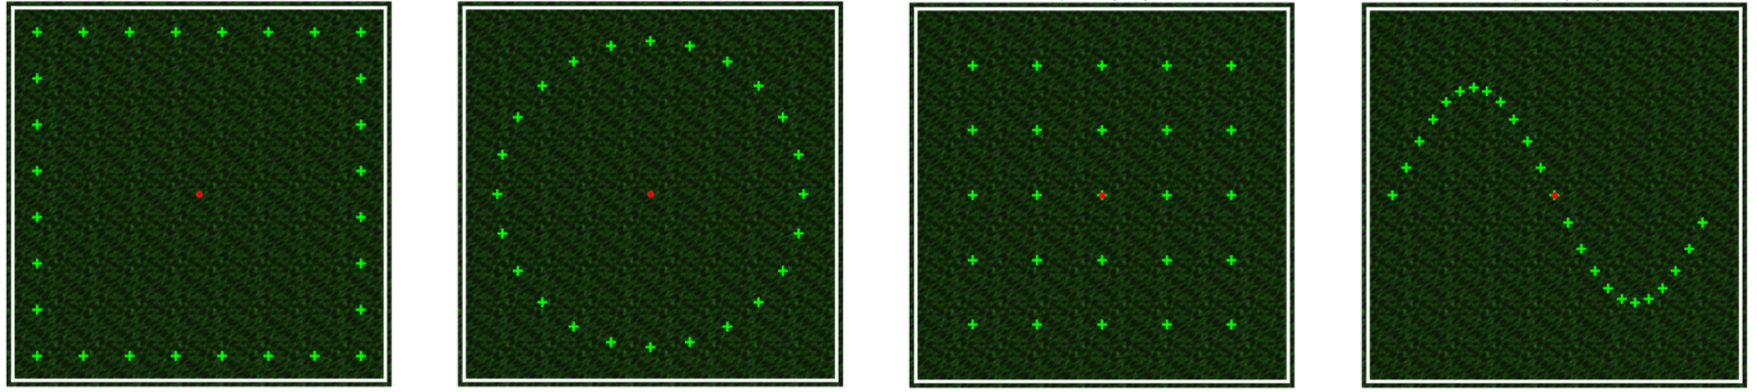
\includegraphics[width=1.0\linewidth]{figuras/medikits-distributions.png}
    \caption{Distribuições espaciais dos \textit{medikits} utilizadas nas análises comportamentais. Da esquerda para a direita, são apresentadas as distribuições em quadrado, círculo, \textit{grid} e seno. Os sinais de ``+'' indicam os \textit{medikits}, enquanto o ponto vermelho indica a posição inicial do agente no episódio.\\
    \textbf{Fonte:} Elaborada pelo autor.}
    \label{fig:medikits-distributions}
\end{figure}

A adoção de distribuições fixas tem como objetivo tornar a análise das trajetórias mais controlada e comparável entre diferentes execuções. Durante o treinamento, os \textit{medikits} surgem em posições aleatórias. Por isso, um agente pode obter bom desempenho sem aprender a se orientar intencionalmente em direção aos recursos, adotando apenas um padrão de deslocamento que ocasionalmente encontra \textit{medikits}. Na distribuição circular, por exemplo, o agente poderia aprender simplesmente a girar ou percorrer uma trajetória circular. Na distribuição em quadrado, poderia permanecer próximo às paredes e coletar recursos incidentalmente ao longo do percurso.

A comparação entre diferentes arranjos permite identificar esse tipo de comportamento estereotipado. Se o agente repetir praticamente a mesma trajetória independentemente da distribuição, a coleta pode ser consequência acidental de uma estratégia geral de movimentação. Se a trajetória variar de acordo com a organização espacial dos \textit{medikits}, haverá evidências de que a política utiliza informações do ambiente para orientar sua navegação. Essa análise não demonstra, por si só, intenção no sentido forte, mas ajuda a distinguir uma política sensível à disposição dos recursos de uma política que apenas os encontra aleatoriamente.

\subsection{Relação entre Recompensa Intrínseca e Precariedade}

Além dessas comparações, será analisado o gráfico de recompensa intrínseca nas execuções que utilizam RND. Esse gráfico será apresentado juntamente com uma medida de precariedade perceptiva, calculada pela razão entre a quantidade de pixels escurecidos pelo glaucoma e a quantidade total de pixels da observação. O valor resultante expressa a porcentagem da visão comprometida em cada instante, variando entre uma observação sem degradação e uma observação amplamente obstruída. A visualização conjunta permitirá examinar como a recompensa intrínseca varia conforme o grau de precariedade perceptiva. A ocorrência de recompensas menores em estados mais degradados e de recompensas maiores em estados menos precários constituirá um indício de que o mecanismo proposto consegue converter a precariedade corporal em um sinal relevante para o aprendizado. Essa análise não será utilizada para comparar diretamente as escalas das diferentes formas de recompensa, mas para avaliar a relação interna entre glaucoma e curiosidade nas configurações baseadas em RND.

\section{Análise Visual da Política Aprendida}

Para complementar a avaliação, pretende-se utilizar técnicas de interpretabilidade visual, como Grad-CAM, discutido na Seção~\ref{subsubsec:gradcam}. O objetivo é identificar quais regiões da observação influenciam as decisões do agente. A Figura~\ref{fig:gradcam-health-gathering} apresenta um exemplo ilustrativo desse tipo de visualização na tarefa \textit{Health-Gathering}. Essa análise é especialmente importante porque o agente atua a partir de imagens e porque a proposta do trabalho depende da relação entre percepção, curiosidade e viabilidade.

A escolha do Grad-CAM segue o mesmo princípio de simplicidade adotado na arquitetura da política. O objetivo não é comparar métodos de interpretabilidade nem obter a explicação visual mais sofisticada possível, mas produzir uma indicação espacial suficientemente clara das regiões da observação que influenciam as decisões do agente. Como a política utiliza camadas convolucionais, o Grad-CAM pode ser aplicado diretamente aos mapas de características da rede e gerar mapas de calor sobrepostos à imagem original, facilitando a interpretação qualitativa do comportamento. Métodos mais sofisticados exigiriam, desnecessariamente, maior custo de processamento. A adoção de uma única técnica simples e compatível com a CNN mantém a análise visual alinhada ao objetivo central do experimento.

\begin{figure}[h!]
    \centering
    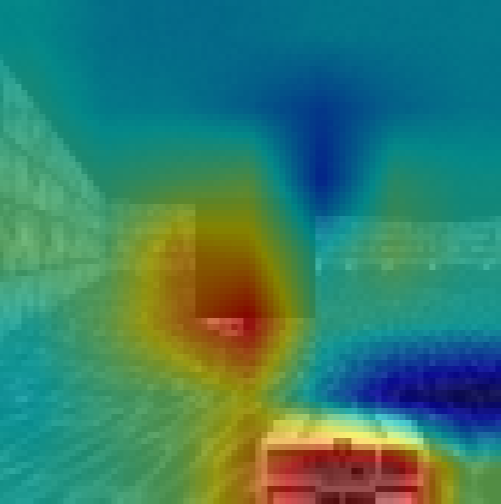
\includegraphics[width=0.6\linewidth]{figuras/gcam-hr.png}
    \caption{Exemplo ilustrativo de mapa de calor inspirado em Grad-CAM aplicado à tarefa \textit{Health-Gathering}. As regiões mais quentes indicam as áreas da observação com maior relevância para a decisão do agente, isto é, aquelas que mais importam na análise visual da política aprendida.\\
    \textbf{Fonte:} Elaborada pelo autor.}
    \label{fig:gradcam-health-gathering}
\end{figure}

Com o Grad-CAM, será possível investigar se o agente direciona sua atenção para elementos relevantes do ambiente, como \textit{medikits}, regiões navegáveis ou obstáculos. Também será possível comparar mapas de ativação em diferentes níveis de degradação perceptiva, buscando compreender como a precariedade visual altera os elementos considerados relevantes pela política.

Essa etapa não tem apenas função técnica, mas também conceitual. Se a proposta busca discutir autonomia e produção de relevância, é necessário analisar não apenas se o agente obtém bom desempenho, mas também como ele utiliza as informações disponíveis para agir. A interpretabilidade visual, portanto, servirá como ferramenta auxiliar para compreender a política aprendida.
